\documentclass[tikz,border=4pt]{standalone}
\usepackage{lmodern}
\usetikzlibrary{arrows.meta,positioning,fit,backgrounds}
\definecolor{io}{HTML}{455A64}
\definecolor{gpu}{HTML}{1565C0}
\definecolor{geo}{HTML}{2E7D32}
\definecolor{ai}{HTML}{6A1B9A}
\definecolor{out}{HTML}{E65100}
\definecolor{web}{HTML}{00838F}
\tikzset{
  box/.style={draw=#1, line width=0.9pt, rounded corners=3pt, fill=#1!7, align=center,
              minimum height=1.2cm, text width=2.7cm, font=\small},
  small/.style={draw=#1, line width=0.7pt, rounded corners=2pt, fill=#1!5, align=center,
                minimum height=0.75cm, text width=2.35cm, font=\scriptsize},
  lbl/.style={font=\scriptsize\itshape, text=black!65, align=center},
  arr/.style={-{Stealth[length=2.2mm]}, line width=0.8pt, draw=black!70},
  both/.style={{Stealth[length=2.2mm]}-{Stealth[length=2.2mm]}, line width=0.8pt, draw=black!70},
  group/.style={draw=#1!60, dashed, rounded corners=5pt, inner sep=7pt},
}
\begin{document}
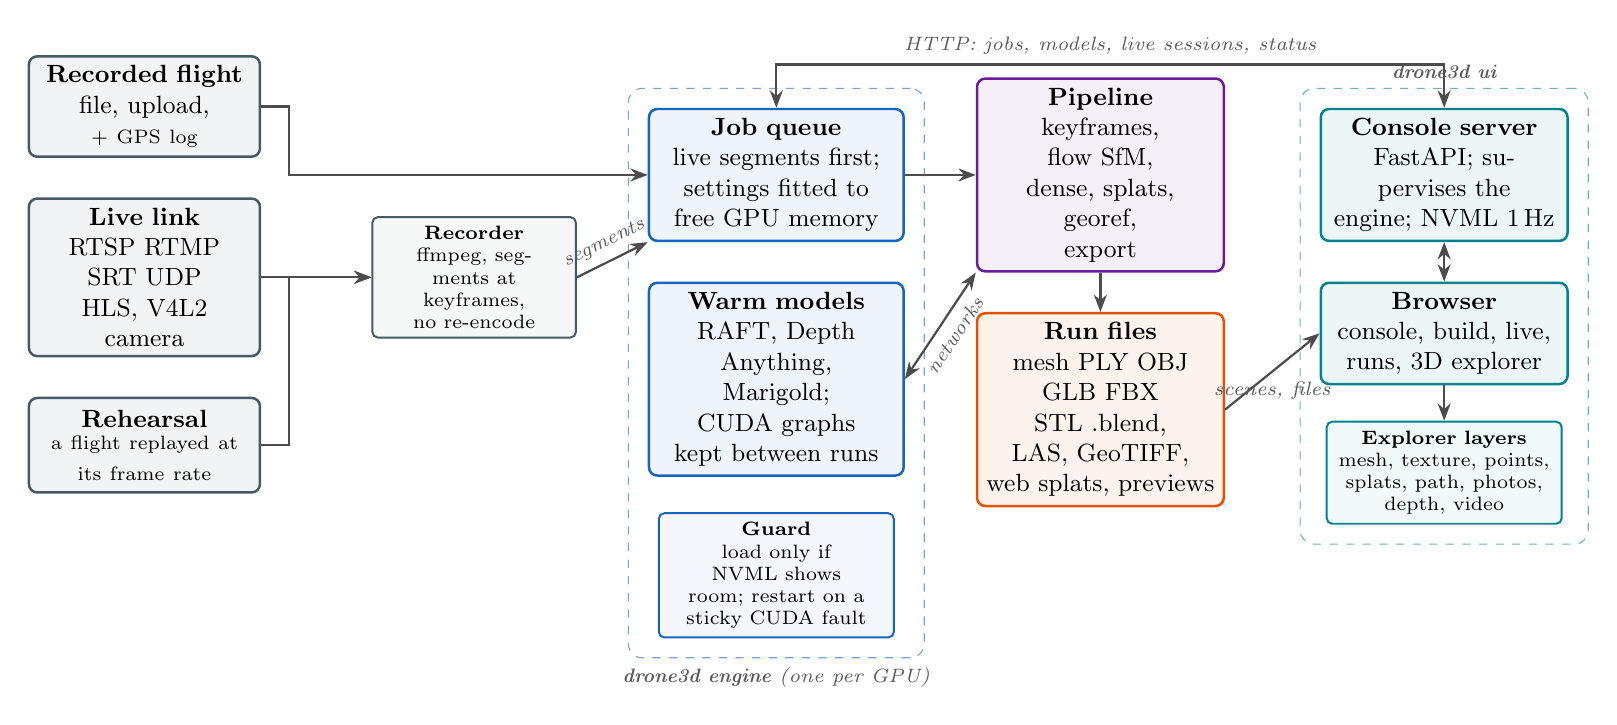
\begin{tikzpicture}[node distance=0.5cm and 0.9cm]
% sources
\node[box=io] (file) {\textbf{Recorded flight}\\ file, upload,\\ \scriptsize + GPS log};
\node[box=io, below=of file] (stream) {\textbf{Live link}\\ RTSP RTMP SRT UDP\\ HLS, V4L2 camera};
\node[box=io, below=of stream] (replay) {\textbf{Rehearsal}\\ \scriptsize a flight replayed at\\ \scriptsize its frame rate};

% engine
\node[small=io, right=1.4cm of stream] (rec) {\textbf{Recorder}\\ ffmpeg, segments at\\ keyframes, no re-encode};
\node[box=gpu, right=of rec, yshift=1.3cm, text width=3.0cm] (queue) {\textbf{Job queue}\\ live segments first;\\ settings fitted to\\ free GPU memory};
\node[box=gpu, below=0.5cm of queue, text width=3.0cm] (cache) {\textbf{Warm models}\\ RAFT, Depth Anything,\\ Marigold; CUDA graphs\\ kept between runs};
\node[small=gpu, below=0.45cm of cache, text width=2.75cm] (guard) {\textbf{Guard}\\ load only if NVML shows\\ room; restart on a\\ sticky CUDA fault};
\node[box=ai, right=of queue, text width=2.9cm] (pipe) {\textbf{Pipeline}\\ keyframes, flow SfM,\\ dense, splats, georef,\\ export};
\node[box=out, below=0.5cm of pipe, text width=2.9cm] (runs) {\textbf{Run files}\\ mesh PLY OBJ GLB FBX\\ STL .blend, LAS, GeoTIFF,\\ web splats, previews};

% console and browser
\node[box=web, right=1.2cm of pipe, text width=2.9cm] (server) {\textbf{Console server}\\ FastAPI; supervises the\\ engine; NVML 1\,Hz};
\node[box=web, below=0.5cm of server, text width=2.9cm] (browser) {\textbf{Browser}\\ console, build, live,\\ runs, 3D explorer};
\node[small=web, below=0.45cm of browser, text width=2.75cm] (layers) {\textbf{Explorer layers}\\ mesh, texture, points,\\ splats, path, photos,\\ depth, video};

\begin{scope}[on background layer]
  \node[group=gpu, fit=(queue)(cache)(guard), label={[lbl]below:\textbf{drone3d engine} (one per GPU)}] (eng) {};
  \node[group=web, fit=(server)(browser)(layers), label={[lbl]above:\textbf{drone3d ui}}] {};
\end{scope}

\draw[arr] (file.east) -- ++(0.35,0) |- (queue.west);
\draw[arr] (stream) -- (rec);
\draw[arr] (replay.east) -- ++(0.35,0) |- (rec.west);
\draw[arr] (rec.east) -- node[lbl, above, sloped] {segments} (queue.south west);
\draw[arr] (queue) -- (pipe);
\draw[both] (cache.east) -- node[lbl, below, sloped] {networks} (pipe.south west);
\draw[arr] (pipe) -- (runs);
\draw[both] (server.north) -- ++(0,0.55) -| node[lbl, pos=0.25, above] {HTTP: jobs, models, live sessions, status} (queue.north);
\draw[arr] (runs.east) -- node[lbl, below] {scenes, files} (browser.west);
\draw[both] (server) -- (browser);
\draw[arr] (browser) -- (layers);
\end{tikzpicture}
\end{document}
